\documentclass[11pt, oneside]{article}   	% use "amsart" instead of "article" for AMSLaTeX format
\usepackage{geometry}                		% See geometry.pdf to learn the layout options. There are lots.
\geometry{letterpaper}                   		% ... or a4paper or a5paper or ...
%\geometry{landscape}                		% Activate for for rotated page geometry
%\usepackage[parfill]{parskip}    		% Activate to begin paragraphs with an empty line rather than an indent
\usepackage{graphicx}				% Use pdf, png, jpg, or eps� with pdflatex; use eps in DVI mode
\usepackage{amsmath}								% TeX will automatically convert eps --> pdf in pdflatex
\usepackage{amssymb}
\setlength{\parindent}{0cm}

\title{Topics in Discrete Math}
\author{Yulong Yang}
%\date{}							% Activate to display a given date or no date

\begin{document}
\maketitle
%\section{}
%\subsection{}

\section{Logic type}

\subsection{propositional}

A proposition is a declarative sentence that is either true or false, but not both. It declares a fact.

Example:

\begin{itemize}
\item ``Washington, D.C., is the capital of the U.S.A.
\item 1 + 1 = 3
\end{itemize}

\subsection{predicate}

Predicate logic usually contains a \textit{variable} and a \textit{predicate}. Without assigning values to the variable, the logic is neither true or false. For example ``$x$ is greater than 3", variable is $x$, and ``is greater than 3" is the predicate, refers to a property the variable could have. If we assign the predicate to be $P(x)$, then it becomes \textit{propositional function} $P$ at $x$. $P(x)$ is a proposition once we assign value to $x$.

Example:
\begin{itemize}
\item $x$ is greater than 3
\item Computer $x$ is under attack
\end{itemize}

\subsection{quantification}

The extent to which a predicate is true over a range of elements (for the variable). Mostly use words like ``all", ``some", etc.

\subsection{logic examples}

\begin{itemize}
\item $p \rightarrow q$: is the proposition ``if $p$ then $q$", which is false iif $p$ is true and $q$ is false [\textit{propositional}]
\item $p \leftrightarrow q$: is the proposition ``$p$ iff $q$", which is true when $p$ and $q$ has the same truth value [\textit{propositional}]
\item $\neg p$: is the proposition ``not $p$", which is true when $p$ is false
\item $\forall xP(x)$: true iif for $P(x)$ is true for every $x$ in the domain [\textit{predicate}]
\end{itemize}

\section{Set}

A set $S$ is closed under addition if for any $x,y \in S$ we have also $x+y \in S$. Also, it is closed under multiplication if $x \times y \in S$.

\section{Regular expression}

\begin{itemize}
\item $\phi$ indicates empty language. In the finite machine, it means start state could be accepted immediately
\item $X+Y$ should expect either $X$ or $Y$, but not both
\item $XY$ should expect first $X$ then $Y$
\item $X^*$ should expect 0 or more $X$s
\item $X^+$ should expect 1 or more $X$s
\end{itemize}

\section{Order notation}

\begin{itemize}
\item $f(n) \in O(g(x))$: there are constants $C$ and $k$ such that $|f(x)| \leq C|g(x)|$ for any $x > k$
\item $f(n) \in \Omega(g(x))$: replace $\leq$ with $\geq$
\item $f(n) \in \Theta(g(x))$: both above two stand correct
\end{itemize}

Master theorem in Figure~\ref{fig:mt}. Use it to solve any recurrence problems.

\begin{figure}[htpb]
\begin{center}
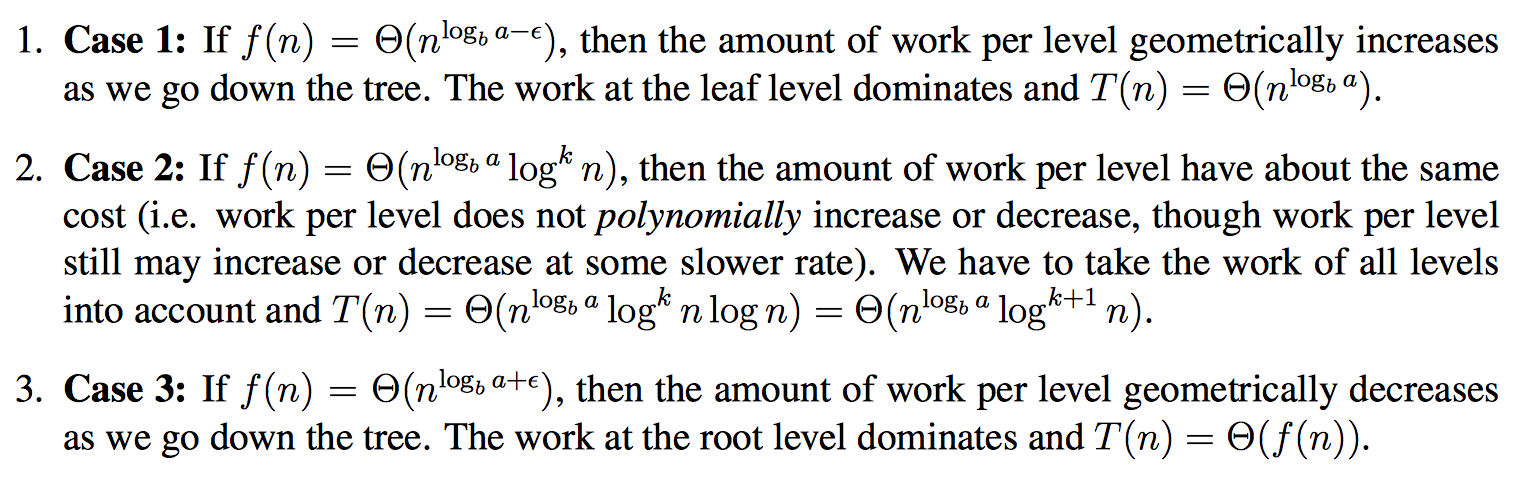
\includegraphics[width=\textwidth]{master.png}
\caption{Master Therorem}
\label{fig:mt}
\end{center}
\end{figure}


\section{Graph}

\subsection{Complete graph}
Complete graph with $n$ vertices is the simple graph that contains exactly one edge between each pair of distinct vertices. Example is in Figure~\ref{fig:complete_graph}.

\begin{figure}[htpb]
\begin{center}
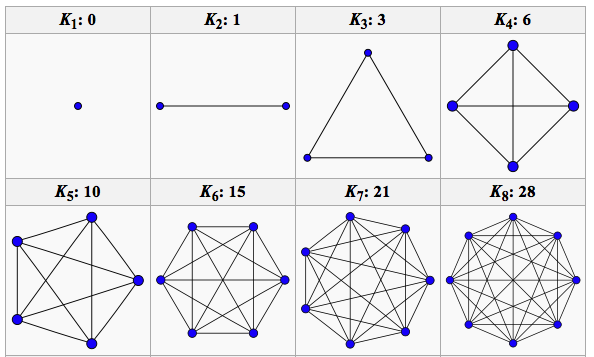
\includegraphics[width=\textwidth]{complete_graph.png}
\caption{Examples of complete graph}
\label{fig:complete_graph}
\end{center}
\end{figure}


\subsection{Planar graph}

\begin{itemize}
\item a graph that could be drawn without any edges crossing (planar representation)
\item Euler's formula: given $e$ edges, $v$ vertices and $r$ regions in a planar representation, we have $r = e - v + 2$
\end{itemize}

\subsection{Bipartite}

\begin{itemize}
    \item $G$ is \textbf{bipartite} if its vertex set $V$ could be divided into 2 \textit{disjoint} sets $V_1$ and $V_2$, s.t. every edge in $G$ connects a vertex in $V_1$ and a vertex in $V_2$, and no edges connect any 2 vertices within either $V_1$ or $V_2$. 
    \item $G$ is bipartite iff it is possible to assign 2 different colors to each vertex s.t. no 2 adjacent vertices are assigned the same color
\end{itemize}

\subsection{Euler path/cycle}

\begin{itemize}
\item a cycle/circuit is a path of length greater than 0 that begins and ends at the same vertex
\item a \textbf{Euler path/cycle} is a simple path/cycle containing every \textit{edge} of $G$ exactly once.
\item a connected multigraph with at least 2 vertices has a Euler cycle iff each of its vertices has even degree (\# of edges, also called \textit{valency})
\item a connected multigraph has an Euler path but not Euler cycle iff it has exactly two vertices with odd degree
\end{itemize}

\subsection{Hamilton path/cycle}

\begin{itemize}
\item a \textbf{Hamilton path/cycle} is a simple path/cycle containing every \textit{vertex} of $G$ exactly once.
\item if $G$ is a simple graph with $n$ vertices with $n\geq 3$ s.t. the degree of every vertex in $G$ is at least $n/2$, then $G$ has a Hamilton cycle.
\item if G with $n$ vertices with $n\geq 3$ s.t. $deg(u)+deg(v)\geq n$ for every pair of nonadjacent vertices $n$ and $v$, then G has a Hamilton cycle.
\end{itemize}
\end{document}
